% arXiv preprint — extended version of the SPIE Medical Imaging submission,
% restructured to the field's (TMI-style) section layout, with the comparative benchmarks.
% Build: tectonic main.tex
\documentclass[11pt]{article}

\usepackage[letterpaper,margin=1in]{geometry}
\usepackage{amsmath,amssymb}
\usepackage{graphicx}
\usepackage{booktabs}
\usepackage[font=small,labelfont=bf]{caption}
\usepackage{microtype}
\usepackage{xcolor}
\definecolor{linkblue}{RGB}{25,60,120}
\usepackage[colorlinks=true,linkcolor=linkblue,citecolor=linkblue,urlcolor=linkblue]{hyperref}

\emergencystretch=1.5em
\renewcommand{\thesection}{\Roman{section}}
\renewcommand{\thesubsection}{\Alph{subsection}}
\makeatletter
\renewcommand{\p@subsection}{\thesection .}
\makeatother

\newcommand{\FDK}{\mathrm{FDK}}
\newcommand{\thetahat}{\hat\theta}
\newcommand{\Pnom}{P_{\mathrm{nom}}}

\title{\bfseries Rigid-Motion Correction in Head Cone-Beam CT with a 3D Flow-Matching
Prior on the Geometry Bridge}

\author{%
Sungho Yun \and Seungryong Cho\\[2pt]
{\normalsize Department of Nuclear and Quantum Engineering,}\\
{\normalsize Korea Advanced Institute of Science and Technology (KAIST), Daejeon 34141, South Korea}}

\date{}

\begin{document}
\maketitle

\begin{abstract}
\noindent
Head motion during a cone-beam CT (CBCT) scan violates the static-object assumption behind
analytic reconstruction, and recovering the per-view rigid poses jointly with the volume is a
blind inverse problem with an exact SE(3) gauge ambiguity. Generative image priors can support
this joint recovery, but a prior trained on clean images must judge heavily corrupted
intermediate reconstructions that lie far outside its training distribution. In this work, we
train a 3D flow-matching prior on a geometry bridge: the family of FDK reconstructions of the
same scan re-simulated with the motion amplitude attenuated linearly to zero. The path
therefore runs from the uncorrected reconstruction to the motion-free FDK by construction, and
its velocity target is analytic, given by the forward projector's exact geometry derivative
carried through the linear FDK. At inference, a blind predictor-corrector loop alternates the
frozen prior, a hash-encoded motion estimator driven by the projector's exact pose gradient,
and a conjugate-gradient data-consistency step. On 30 held-out CQ500 patients with
10\,mm\,/\,10$^\circ$ peak-to-peak Akima motion, the method improves every patient, raising
PSNR from 23.3 to 36.7\,dB and SSIM from 0.55 to 0.978, and reducing the reprojection error
from 6.12 to 0.28\,mm, in 9.3 minutes per patient. We further report a paired comparison on
identical data against the two published paradigms in this setting, both retrained on our
training patients: a learned-metric autofocus method (Thies et al., IEEE TMI 2025) and the
wavelet diffusion prior of JRM-ADM run inside our unchanged loop. The recovered motion is
accurate enough that the FDK at the estimated poses is nearly indistinguishable from the FDK
at the true poses (SSIM 0.980 against this oracle, versus 0.845 for the autofocus baseline),
and the flow-matching prior is worth $+8.5$\,dB over the diffusion prior under an identical
loop, with a pixel-linear bridge ablation attributing $+1.4$\,dB to the physics-consistent
bridge itself. The final iterate surpasses even the motion-free FDK reference by 3.5\,dB,
indicating that the reconstruction operator, not residual motion, is the limiting factor.
\end{abstract}

\section{Introduction}
\label{sec:intro}

Cone-beam CT serves head and neck imaging in image-guided radiotherapy, interventional suites
and point-of-care settings. A scan takes tens of seconds, and head motion within that window
violates the static-object assumption behind analytic reconstruction, producing streaks and
blur severe enough to compromise diagnostic value. Because the skull is rigid, the motion is
well described by a six-degree-of-freedom (6-DoF) pose per view, a parameterization that is
compact but difficult to recover from the projections alone.

The problem is blind. Writing the scan as $y = A_{P(\theta)}x$, neither the volume $x$ nor the
trajectory $\theta$ is known, and the measurement is bilinear in the operator-image pair:
estimating the geometry requires a clean image, while reconstructing one requires the correct
geometry. The joint objective is therefore non-convex, and it carries an exact SE(3) gauge: a
global rigid transform applied to both object and orbit leaves the sinogram unchanged, so
$\theta$ is identifiable only up to a rigid transform.

Existing approaches fall into two main families. Autofocus methods recover $\theta$ by
optimizing an image-quality surrogate of the reconstruction, classically a sharpness or
entropy criterion~\cite{sisniega17}. Learning-based variants replace the hand-crafted
surrogate with a trained quality metric: Thies et al.~\cite{thies25} regress a voxelized
visual-information-fidelity (VIF) map and drive a gradient-based search on spline motion
parameters through a differentiable backprojector, and Huang et al.~\cite{huang22} regress a
scalar quality score with a similar aim, while Ko et al.~\cite{ko21} map the corrupted volume
directly to a clean one without recovering motion. These methods estimate motion accurately
and quickly, but the image they return is an analytic reconstruction at the estimated poses
and inherits the limits of that operator. The second family inserts a generative model of
clean CT into an iterative solver, following the plug-and-play framework~\cite{pnp13} and its
diffusion-based successors~\cite{dds24}. For rigid-motion head CBCT specifically, the closest
published method is JRM-ADM~\cite{depaepe25}, which alternates a wavelet-domain diffusion
prior (W3DM~\cite{wdm24}) with a weighted-least-squares data step and a blind B-spline motion
update on CQ500 data. A structural difficulty is shared by this family: the generative path of
such a prior runs from Gaussian noise to a clean image by construction, so the prior never
sees the partially corrected, artifact-laden reconstructions that a blind correction loop
actually visits, and must be reached through noising heuristics at every iteration.

Flow matching~\cite{lipman23} removes this restriction: the endpoints of the learned
transport, and the interpolation between them, can be prescribed
freely~\cite{indi23,albergo23,i2sb23}. We use this freedom to train the prior on a geometry
bridge, the family of FDK reconstructions of the same scan re-simulated with the motion
amplitude attenuated linearly to zero. The path then runs from the uncorrected reconstruction
at $t{=}0$, where inference starts, to the motion-free reconstruction at $t{=}1$. Its
intermediate states are the images a correction loop passes through, so the prior remains
well-defined at every iterate and supplies the update direction that a joint recovery of image
and motion requires. Fig.~\ref{fig:manifold} illustrates the idea: a clean-image prior must
carry the loop's off-manifold states back to a path it was never trained on, whereas the
geometry bridge makes those states the training path itself. Bridge-type models of this kind
have been applied to image restoration and low-dose CT, but to our knowledge not to CT
rigid-motion correction.

\begin{figure}[t]
\centering
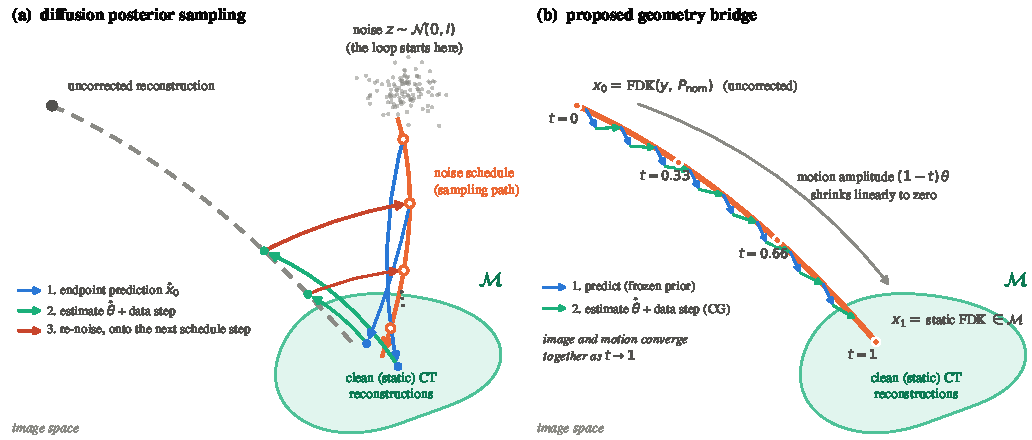
\includegraphics[width=0.95\textwidth]{fig0_manifold.pdf}
\caption{Concept of the proposed method. (a) A generative prior of clean images transports
Gaussian noise to the clean-reconstruction manifold $\mathcal{M}$ along a fixed path; the
partially corrected reconstructions that a blind correction loop actually visits lie outside
its training distribution and can only be reached through re-noising heuristics. (b) The
geometry bridge makes that family of states the training path itself: $x_t$ is the FDK
reconstruction of the same scan carrying $(1-t)$ of the motion, the path ends on the static
FDK by construction, and the regression target is the analytic operator tangent
$dx_t/dt$. Inference walks the bridge: the frozen prior advances the image along the learned
velocity, the motion is refit on the improved image, and the data-consistency step returns
the iterate to the bridge, so the image and the motion converge together as $t\to1$.}
\label{fig:manifold}
\end{figure}

The contributions of this work are as follows. (1) A 3D flow-matching prior on the geometry
bridge, whose velocity target is analytic: FDK is linear in the sinogram and the nominal
geometry is fixed, so the bridge tangent is the forward projector's exact geometry derivative
carried through the reconstruction operator, with no finite differencing. (2) A blind
predictor-corrector loop in which the frozen prior, a hash-encoded motion estimator and a
plug-and-play data step reinforce one another, evaluated on 30 held-out patients under a fully
specified scan geometry and gauge convention. (3) A paired comparison on identical data
against the two published paradigms in this setting, the learned-metric autofocus of Thies et
al.~\cite{thies25} and the diffusion prior of JRM-ADM~\cite{depaepe25}, both retrained on our
training patients, together with a pixel-linear bridge ablation that isolates the contribution
of the physics-consistent bridge. An earlier version of this work was presented in a
conference submission; this paper adds the comparative evaluation.

\section{Methods}
\label{sec:method}

\subsection{Problem formulation}
\label{sec:forward}

Let $x$ denote the attenuation volume and $y$ the log-transformed projections acquired over
$V$ views along the nominal circular orbit $\Pnom$. Patient motion displaces view $v$ by a
rigid pose $\theta_v \in \mathbb{R}^6$ (axis-angle rotation and translation), so the true
acquisition geometry is $P(\theta)[v] = \Pnom[v]\,T(\theta_v)$, where $T(\cdot)$ maps a pose
to its rigid transform and $\theta \in \mathbb{R}^{V\times 6}$ collects the per-view poses
into one motion trajectory. The scan is $y = A_{P(\theta)}x$, with $A_P$ the cone-beam forward
projector at geometry $P$. We seek the volume and the motion jointly,
\begin{equation}
\min_{x,\,\theta}\ \tfrac12\,\|A_{P(\theta)}x - y\|_2^2 \;+\; \lambda\,\mathrm{TV}(x)
\;+\; \mathcal{R}(x),
\label{eq:objective}
\end{equation}
where the first term enforces consistency with the measured projections at the current
geometry estimate, the total-variation term suppresses the streaks that survive an imperfect
geometry, and $\mathcal{R}$ is the learned flow-matching prior of Sec.~\ref{sec:bridge},
which enters the iteration through its velocity field.

Two structural facts inform the design. First, per-view translation along the beam axis is
nearly unobservable in cone-beam geometry, since it acts only through magnification; we
therefore report the observable translation component separately rather than a single
translation RMSE. Second, because of the SE(3) gauge, volumes must be rigidly aligned to the
ground truth before image metrics are computed, and motion accuracy must be quoted under an
explicit gauge convention (Sec.~\ref{sec:protocol}).

\subsection{Flow-matching prior on the geometry bridge}
\label{sec:bridge}

Flow matching learns a velocity field $v_\phi(x,t)$ that transports one distribution into
another along a prescribed path, by regressing $v_\phi(x_t,t)$ onto the path tangent
$dx_t/dt$. We set that path to the geometry bridge sketched in Fig.~\ref{fig:manifold}(b)
and shown with actual reconstructions in Fig.~\ref{fig:method}(a): at flow time
$t$ the motion is scaled down to $(1-t)\theta$, the scan is re-simulated at that reduced
motion, and reconstructed at the nominal geometry,
\begin{equation}
y_t = A\!\left(x;\ \Pnom T((1-t)\theta)\right), \qquad
x_t = \FDK(y_t,\ \Pnom).
\label{eq:bridge}
\end{equation}
Because the bridge scales the axis-angle vector, the motion carried by $y_t$ is exactly
$(1-t)\theta$, and the path sweeps the motion amplitude linearly to zero. Every point on the
path is an FDK reconstruction of the same patient scanned with progressively less motion, and
both endpoints follow by construction, with no correction term. At $t{=}0$ the re-simulated
scan is the measured one, so $x_0 = \FDK(y,\Pnom)$ is exactly the uncorrected reconstruction
from which inference starts. At $t{=}1$ the scan is motion-free and traverses the nominal
circular, equiangular orbit, so $x_1$ is exactly the static FDK, the best reconstruction this
scanner and this operator can produce of a still patient. Both identities hold to float
precision.

\begin{figure}[t]
\centering
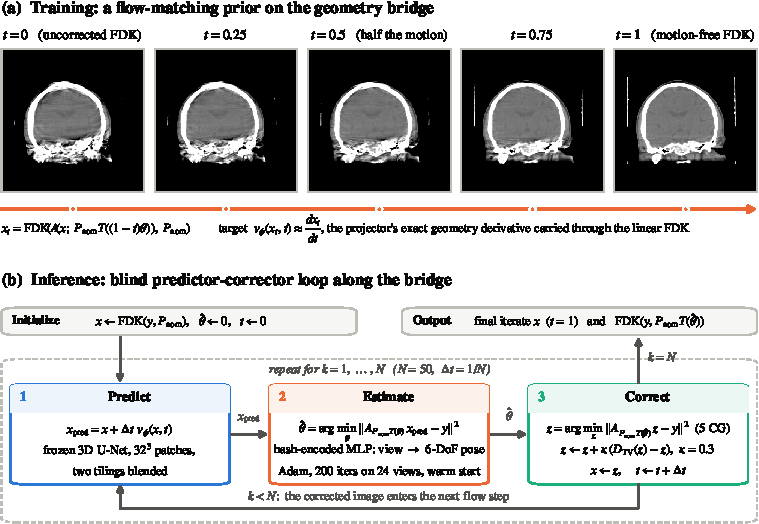
\includegraphics[width=0.92\textwidth]{fig1_method.pdf}
\caption{(a) The geometry bridge: each panel is an actual FDK reconstruction of a scan
re-simulated with exactly $(1-t)$ of the true motion, so the path ends on the motion-free
static FDK by construction. The velocity target $dx_t/dt$ is the forward projector's exact
geometry derivative carried through the linear FDK. (b) One step of the blind inference loop:
the frozen prior moves the image, the motion is refit on the improved image, and a
plug-and-play data step enforces consistency at the new estimate.}
\label{fig:method}
\end{figure}

A key property of this construction is that the tangent is available in closed form. FDK is
linear in the sinogram and $\Pnom$ does not depend on $t$, so the time derivative passes
through the reconstruction operator:
\begin{equation}
\frac{dx_t}{dt} = \FDK\!\left(\frac{\partial y_t}{\partial t},\ \Pnom\right),
\qquad
\frac{\partial y_t}{\partial t}
= -\,\frac{\partial A}{\partial P}\Big[x;\ \Pnom T((1-t)\theta)\Big]\cdot \Pnom\,\dot{T}\,\theta,
\label{eq:tangent}
\end{equation}
where $\partial A/\partial P$ is the forward projector's exact geometry derivative and
$\dot T$ the axis-angle generator. No finite differencing is needed, which matters in
practice: we measured single-precision central differences of this path to bottom out near
2\% relative error in the image domain, because the ramp filter amplifies cancellation noise,
whereas the transcribed exact derivative kernel agrees with a double-precision autograd
reference to $2.8\times10^{-6}$. The cost is one extra forward projection and one extra
backprojection per training sample. The loss is $\|v_\phi(x_t,t) - dx_t/dt\|^2$ with
$t\sim\mathcal{U}[0,1]$. The velocity field is a 3D U-Net on $32^3$ patches;
following~\cite{yang25}, each patch carries four conditioning channels besides its own
intensities, namely a downsampled view of the whole volume and three absolute coordinate
maps, supplying the global context a $32^3$ receptive field cannot see.

One design choice deserves explanation. This bridge attenuates the motion in the measurement,
so its intermediate images are reconstructions of a patient who moved less; inference, by
contrast, always reconstructs one fixed measured scan at a partially corrected geometry. We
measured the two families to differ by at most 1.1\% RMS of the image range at matched $t$ on
held-out patients. The alternative construction, reconstructing the fixed scan at a partially
corrected geometry, does not end on the static FDK: per-view motion breaks the circular
equiangular orbit assumed by the analytic weighting, and the bare endpoint falls 1--3\,dB
short of the static FDK, which would require a hand-tuned endpoint correction. We accept the
slightly looser match to the inference trajectory in exchange for a clean endpoint.

\subsection{Blind posterior loop}
\label{sec:loop}

Inference (Fig.~\ref{fig:method}(b)) starts from $x = \FDK(y,\Pnom)$ and $\thetahat = 0$, and
takes $N{=}50$ Euler steps along the bridge, each a Gauss-Seidel sweep of three updates.

\textbf{Predict.} The frozen prior moves first, $x_{\mathrm{pred}} = x + \Delta t\,
v_\phi(x,t)$, evaluated patch-wise and blended over two tilings.

\textbf{Estimate.} The motion is refit on the image the prior just improved, taking
$\thetahat$ to minimize $\|A_{\Pnom T(\theta)}\,x_{\mathrm{pred}} - y\|_2^2$ by
backpropagating through the projector's exact geometry gradient. The poses are not free
per-view parameters: an MLP reads the normalized view index through a multiresolution hash
encoding~\cite{mueller22} and outputs the 6-DoF pose, so the trajectory is a continuous
function of the view with no explicit smoothness penalty. Adam optimizes the encoder and MLP
weights, and its state persists across flow steps, so each step warm-starts from the last.
Fitting on $x_{\mathrm{pred}}$ rather than $x$ is what lets the estimate improve from step to
step, since the fit is only as accurate as the image it is made against.

\textbf{Correct.} A plug-and-play forward-backward step enforces consistency at $\thetahat$
through five conjugate-gradient (CG) iterations on $\min_z \|A_{\thetahat}z - y\|^2$,
followed by a relaxed total-variation update $z \leftarrow z + \kappa(\mathrm{TV}(z) - z)$. A
filtered solve rather than a plain adjoint step is important here: the adjoint direction is
dominated by low frequencies, whereas the benefit of a better $\thetahat$ lies in streaks and
edges. The output becomes the image the prior advances at the next flow time, so the image
and the motion converge together as $t$ runs to 1. The loop returns both $\FDK(\thetahat)$
and the final iterate $x_t$, and we report both.

\subsection{Implementation details}
\label{sec:impl}

The prior was trained for 500k iterations (AdamW, cosine learning rate
$10^{-4}\!\to\!10^{-6}$, EMA 0.999, fp16, 64 patches per batch). All projection and
backprojection operations use the modular-beam projector of LEAP~\cite{leap23}, a
differentiable CT library, pinned to its Joseph kernel so that a single operator serves
simulation, the estimator gradient and the data step; the bridge tangent and the pose gradient
are exact derivatives of that same kernel. The estimator runs 200 Adam iterations per flow
step on 24 randomly drawn views, warm-started from the previous step, at half volume
resolution until $t=0.5$.

\section{Experiments}
\label{sec:setup}

\subsection{Data and simulation setup}
\label{sec:data}

We use the CQ500 head CT collection~\cite{cq500}, 343 patients split into 150 training, 50
validation and 143 test patients, reconstructed at $256^3$ with 1\,mm voxels. Projections are
simulated on a native $612^3$ grid at 0.42\,mm, finer than the inversion grid to avoid an
inverse crime, through the standard head-CBCT geometry of~\cite{thies25}: source-isocenter
distance 785\,mm, source-detector distance 1200\,mm, a $700\times500$ detector at 0.64\,mm
pixel pitch, and 360 views over a full turn. Per-view motion follows the motion model
of~\cite{thies25}, a zero-centred Akima spline~\cite{akima70} through 10 random nodes per
DoF. Training draws per-DoF amplitudes up to 15\,mm\,/\,20$^\circ$; evaluation uses a fixed
10\,mm\,/\,10$^\circ$ pattern per patient.

All amplitudes in this paper are peak-to-peak. This convention needs stating because the
literature is inconsistent under the same words: the released sampler of~\cite{thies25} draws
spline nodes in $\pm A/2$ when the paper says amplitude $A$, so their evaluation setting of
5\,mm\,/\,5$^\circ$ is 5\,mm peak-to-peak (initial median RPE around 3\,mm, consistent with
their reported value), whereas JRM-ADM~\cite{depaepe25} draws nodes in $\pm5$, which is
10\,mm peak-to-peak and exactly our evaluation setting. Our evaluation is therefore at twice
the amplitude of~\cite{thies25}, which we keep deliberately as the harder problem.

\subsection{Evaluation protocol}
\label{sec:protocol}

Following the 30-patient protocol of~\cite{thies25}, we score 30 patients from the held-out
test split, one motion pattern each. Because of the SE(3) gauge, volumes are rigidly aligned
to the ground truth before PSNR and SSIM are computed. Motion accuracy is measured by the
reprojection error (RPE)~\cite{thies25}, the mean detector displacement induced by the pose
error over 300 points at radii 25, 50 and 100\,mm, quoted in two conventions: raw, the
definition of~\cite{thies25}, and zero-centred, which removes the mean pose offset. The
zero-centred value uses no ground truth and corresponds to the gauge in which the motion
simulators of all compared methods already write $\theta$; both values are reported wherever
they differ.

In addition to the parameter-domain RPE, we assess motion accuracy in the image domain by
comparing the reconstruction at the estimated poses against the same operator's
reconstruction at the true poses, $\FDK(\theta_{\mathrm{true}})$. This oracle is the proper
ceiling for any FDK-type output: even a perfect motion estimate cannot reproduce the
motion-free scan, because per-view motion breaks the circular equiangular orbit assumed by
the analytic weighting. When this ceiling is used to compare across methods with different
reconstruction operators, both reference reconstructions use the standard weighting (cosine
weight, ramp filter, uniform angular weight), so that implementation-specific weighting
choices do not enter the reference. All statistical comparisons are paired: every method sees
identical (patient, motion draw, simulated sinogram) triples, differences are tested with the
two-sided Wilcoxon signed-rank test over the 30 patients, and the pairing is verified on the
stored true motion of every run.

We also verified that the gauge is genuinely quotiented rather than approximately fitted.
The rigid alignment is converged: extending it from 200 to 800 iterations, or fitting it on
a body region of interest instead of the measured region, changes the scores by less than
0.01\,dB and $10^{-4}$ SSIM. And the transform it recovers is the physical gauge: on a
representative case the image-domain alignment finds 1.1\,mm\,/\,$0.8^\circ$ where the SE(3)
gauge fitted directly to $\thetahat$ in the pose domain is 1.5\,mm\,/\,$0.7^\circ$.

\subsection{Comparison methods}
\label{sec:baselines}

\paragraph{Learned-metric autofocus (Thies et al.~\cite{thies25}).}
The published method regresses a voxelized VIF quality map of a perturbed reconstruction and
optimizes 30 spline nodes per DoF with 100 gradient-descent iterations through a
differentiable backprojector, at 2\,mm resolution, with the final reconstruction at 1\,mm.
Only the backprojector of~\cite{thies25} is publicly released, so the motion model, the
VIF target, the quality network and the optimizer were reimplemented following the paper,
and the quality network was trained on our 150 training patients under their protocol. At the
operating point reported in~\cite{thies25}, the reimplementation reproduces the published
image-quality behaviour (SSIM $0.85\to0.93$ against the motion-free reconstruction, versus
their $0.83\to0.94$) with a somewhat higher residual RPE (1.16\,mm versus their 0.61\,mm),
concentrated out of the source rotation plane; its motion accuracy should therefore be read
as a slightly conservative estimate of the original. The baseline is scored with its own
reconstruction operator throughout.

\paragraph{Diffusion prior of JRM-ADM~\cite{depaepe25}.}
The full JRM-ADM pipeline targets sparse-view acquisitions on a $160\times192\times192$ grid,
so a whole-pipeline transplant would confound the prior, the solver, the grid and the
protocol. Our primary comparison therefore swaps only the prior: their wavelet-domain
diffusion model (W3DM~\cite{wdm24}) is retrained on the same 150 training patients (300k
iterations, their noise schedule) and run inside our unchanged loop, with the same estimator,
the same CG data step, the same schedule and the same measurements. Each network is used in
its native parameterization: the diffusion prior receives a renoised copy of the current
iterate (an SDEdit-style adapter~\cite{sdedit22}; the loop state itself is never noised), and
its $\hat x_0$ prediction is consumed as a fractional step in the manner of
InDI~\cite{indi23}. The renoise level $t_{\max}$, the adapter's only free parameter, was
swept over $\{50,150,300,500,700\}$ on validation patients; the result is a plateau of
30--31\,dB across the sweep, and $t_{\max}{=}300$, the SSIM maximum, was frozen before
touching the test cohort.

\paragraph{Bridge ablation (pixel-linear bridge).}
An identically configured prior, with the same U-Net, conditioning, $t$-sampling and 500k
recipe, trained on the pixel-linear bridge $x_t = (1-t)x_0 + t\,x_1$ between the same two
endpoints, whose velocity target is the constant $x_1 - x_0$. This isolates the contribution
of the physics-consistent bridge shape, a curve through actual FDK reconstructions with the
analytic operator tangent, from all other components.

\section{Results}
\label{sec:results}

\subsection{Motion compensation performance}
\label{sec:results-main}

\begin{table}[t]
\centering
\caption{Image quality on 30 held-out CQ500 patients with Akima motion at
10\,mm\,/\,10$^\circ$ peak-to-peak. PSNR and SSIM are computed against the ground-truth
volume after rigid alignment (mean $\pm$ standard deviation). All methods were retrained on
the same 150 training patients and evaluated on identical (patient, motion, sinogram)
triples. The last two rows are references, not competing methods.}
\label{tab:main}
\begin{tabular}{lcc}
\toprule
Method & PSNR (dB) & SSIM \\
\midrule
Uncorrected FDK & 23.29 $\pm$ 0.93 & 0.546 $\pm$ 0.035 \\
Thies et al.~\cite{thies25} & 30.62 $\pm$ 1.37 & 0.754 $\pm$ 0.040 \\
W3DM prior~\cite{depaepe25} in our loop & 28.15 $\pm$ 2.34 & 0.877 $\pm$ 0.038 \\
FM prior, pixel-linear bridge (ablation) & 35.29 $\pm$ 2.28 & 0.966 $\pm$ 0.015 \\
Proposed, FDK($\thetahat$) & 31.80 $\pm$ 0.76 & 0.753 $\pm$ 0.032 \\
\textbf{Proposed, $x_t$ (final iterate)} & \textbf{36.66 $\pm$ 1.58} & \textbf{0.978 $\pm$ 0.008} \\
\midrule
\emph{Reference:} FDK at true motion & 33.34 $\pm$ 1.35 & 0.773 $\pm$ 0.032 \\
\emph{Reference:} motion-free FDK & 33.11 $\pm$ 1.50 & 0.832 $\pm$ 0.032 \\
\bottomrule
\end{tabular}
\end{table}

Table~\ref{tab:main} summarizes image quality over the cohort. The uncorrected
reconstruction sits at 23.29\,dB\,/\,0.546 SSIM; the final iterate $x_t$ reaches
36.66\,dB\,/\,0.978, a gain of 13.4\,dB and 0.43 SSIM, and improves every one of the 30
patients (Fig.~\ref{fig:quant}(a)). The mean reprojection error falls from 6.12\,mm to
0.28\,mm (Fig.~\ref{fig:quant}(b)); the residual pose error is $0.27^\circ$ rotation RMSE
(from $4.18^\circ$ uncompensated) and 0.080\,mm in the observable translation component
(from 3.30\,mm), both after quotienting the SE(3) gauge.

Two comparisons in Table~\ref{tab:main} locate the remaining error. First, the gap between
FDK($\thetahat$) and the FDK at the true motion is small (Sec.~\ref{sec:results-motion}
quantifies it directly), so little is left to gain from a better geometry estimate. Second,
$x_t$ exceeds not only FDK($\thetahat$) by 4.9\,dB but also the motion-free FDK reference by
3.5\,dB and 0.146 SSIM. The analytic reconstruction operator, not residual motion, is the
binding constraint, and $x_t$ bypasses it because the same loop also regularizes the
cone-beam and finite-view artifacts that FDK leaves behind. For this reason we regard the
final iterate, rather than an analytic reconstruction, as the primary deliverable. Inference
takes 9.3 minutes per patient on one RTX A6000 GPU, of which roughly 80\% is spent in the
motion estimator.

\begin{figure}[t]
\centering
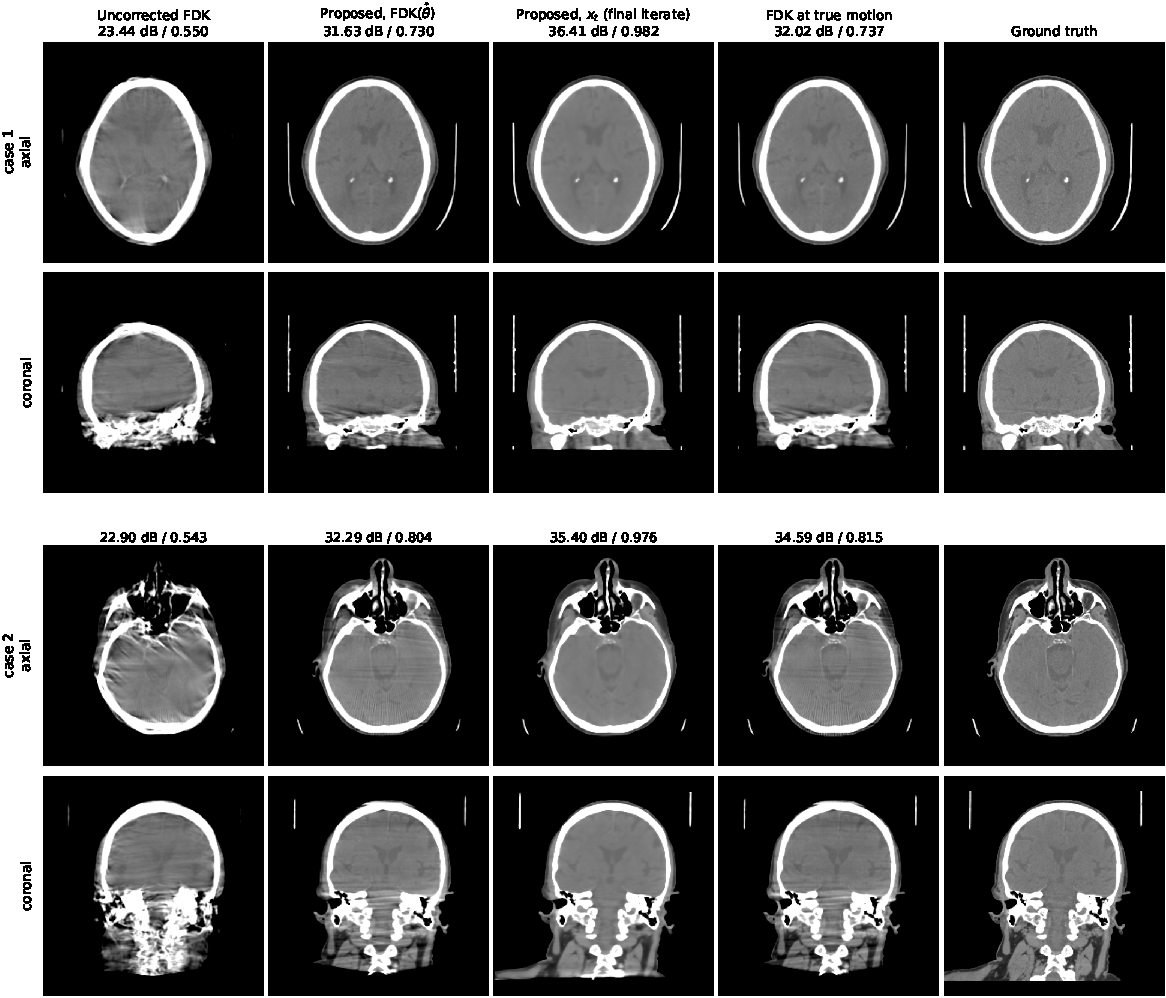
\includegraphics[width=0.82\textwidth]{fig_ours_qual.pdf}
\caption{Two representative test patients at 10\,mm\,/\,10$^\circ$ motion, brain window
(level 40\,/\,width 420\,HU); volumes are rigidly aligned to the ground truth before display,
and labels give PSNR\,/\,SSIM against the ground-truth volume. In both cases
FDK($\thetahat$) is visually indistinguishable from the FDK reconstructed with the
ground-truth motion, and both retain artifacts that only $x_t$ removes.}
\label{fig:images}
\end{figure}

\begin{figure}[t]
\centering
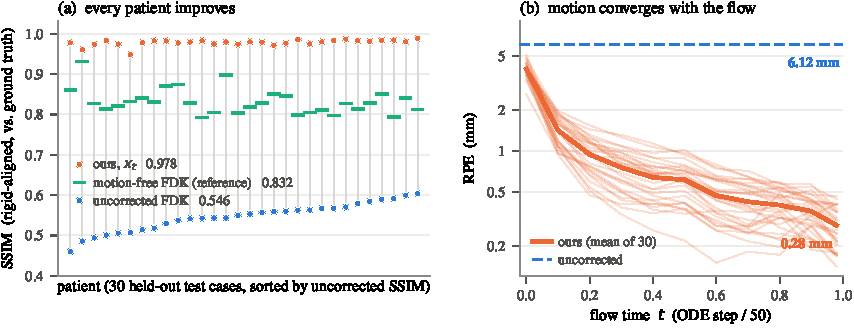
\includegraphics[width=0.7\textwidth]{fig3_quant.pdf}
\caption{Cohort results over 30 held-out patients. (a) Per-patient SSIM; grey stems join each
patient's uncorrected and corrected score. (b) Reprojection error against flow time (thin:
individual patients).}
\label{fig:quant}
\end{figure}

\subsection{Motion estimation accuracy}
\label{sec:results-motion}

\begin{table}[t]
\centering
\caption{Motion estimation accuracy on the same 30 patients. RPE is reported raw (the
definition of~\cite{thies25}) and zero-centred (mean pose offset removed; no ground truth
used). The last column scores the reconstruction at the estimated poses against the same
operator's reconstruction at the true poses, FDK($\theta_{\mathrm{true}}$), with standard
weighting and after rigid alignment; a value of 1 would mean the recovered motion is
indistinguishable from the true motion through the reconstruction operator.}
\label{tab:motion}
\small
\begin{tabular}{lccc}
\toprule
Method & RPE raw (mm) & RPE zero-centred (mm) & SSIM vs.\ FDK($\theta_{\mathrm{true}}$) \\
\midrule
No compensation & 6.12 $\pm$ 0.66 & 6.12 $\pm$ 0.66 & --- \\
Thies et al.~\cite{thies25} & 2.34 $\pm$ 0.51 & 2.26 $\pm$ 0.52 & 0.845 $\pm$ 0.048 \\
W3DM prior~\cite{depaepe25} in our loop & 2.23 $\pm$ 0.63 & 1.35 $\pm$ 0.51 & 0.883 $\pm$ 0.035 \\
FM prior, pixel-linear bridge & 1.69 $\pm$ 0.52 & 0.42 $\pm$ 0.17 & 0.965 $\pm$ 0.017 \\
\textbf{Proposed} & \textbf{1.73 $\pm$ 0.51} & \textbf{0.28 $\pm$ 0.09} &
\textbf{0.980 $\pm$ 0.008} \\
\bottomrule
\end{tabular}
\end{table}

Table~\ref{tab:motion} compares the recovered motion itself, in the parameter domain (RPE)
and in the image domain (similarity of the FDK at the estimated poses to the FDK at the true
poses). Three observations follow.

First, the proposed loop recovers the motion to 0.28\,mm zero-centred RPE, and the
reconstruction at the estimated poses reaches 0.980 SSIM against the oracle reconstruction at
the true poses. In other words, passing the estimated trajectory through the reconstruction
operator produces a volume nearly indistinguishable from the one the true trajectory would
produce; this is direct evidence that the motion extraction itself is accurate, independent
of any learned component in the final image. The corresponding value for the autofocus
baseline is 0.845, lower on every one of the 30 patients ($p=1.9\times10^{-9}$). Raw RPE
shows the same ordering (1.73 versus 2.34\,mm, ours lower on 24/30, $p=1.2\times10^{-5}$);
zero-centring changes ours substantially (0.28\,mm) but theirs little (2.26\,mm), because a
short descent from zero initialization accumulates no global pose offset, while our estimate
carries a genuine gauge component that the zero-centred convention legitimately removes.

Second, one caveat supports the use of the oracle-referenced score. Against the ground-truth
volume, the output of the autofocus baseline (0.754, Table~\ref{tab:main}) exceeds its own
oracle reconstruction at the true motion (0.709 with standard weighting): an autofocus
objective optimizes the appearance of the reconstruction rather than the geometry, and can
surpass its operator's oracle on appearance metrics. Comparisons of motion accuracy through
appearance metrics alone are therefore not conclusive, and we regard the oracle-referenced
column of Table~\ref{tab:motion} as the decisive one.

Third, motion accuracy in the unified loop degrades monotonically with prior quality, in both
domains: 0.28, 0.42 and 1.35\,mm zero-centred RPE, and 0.980, 0.965 and 0.883
oracle-referenced SSIM, for the physics bridge, the linear bridge and the W3DM prior,
respectively. The estimator, the data step and the schedule are identical across these three
rows, so the differences are attributable to the intermediate images each prior supplies to
the estimator. This coupling is analysed further in the next subsection.

\subsection{Effect of the prior and of the bridge}
\label{sec:results-arms}

\begin{figure}[t]
\centering
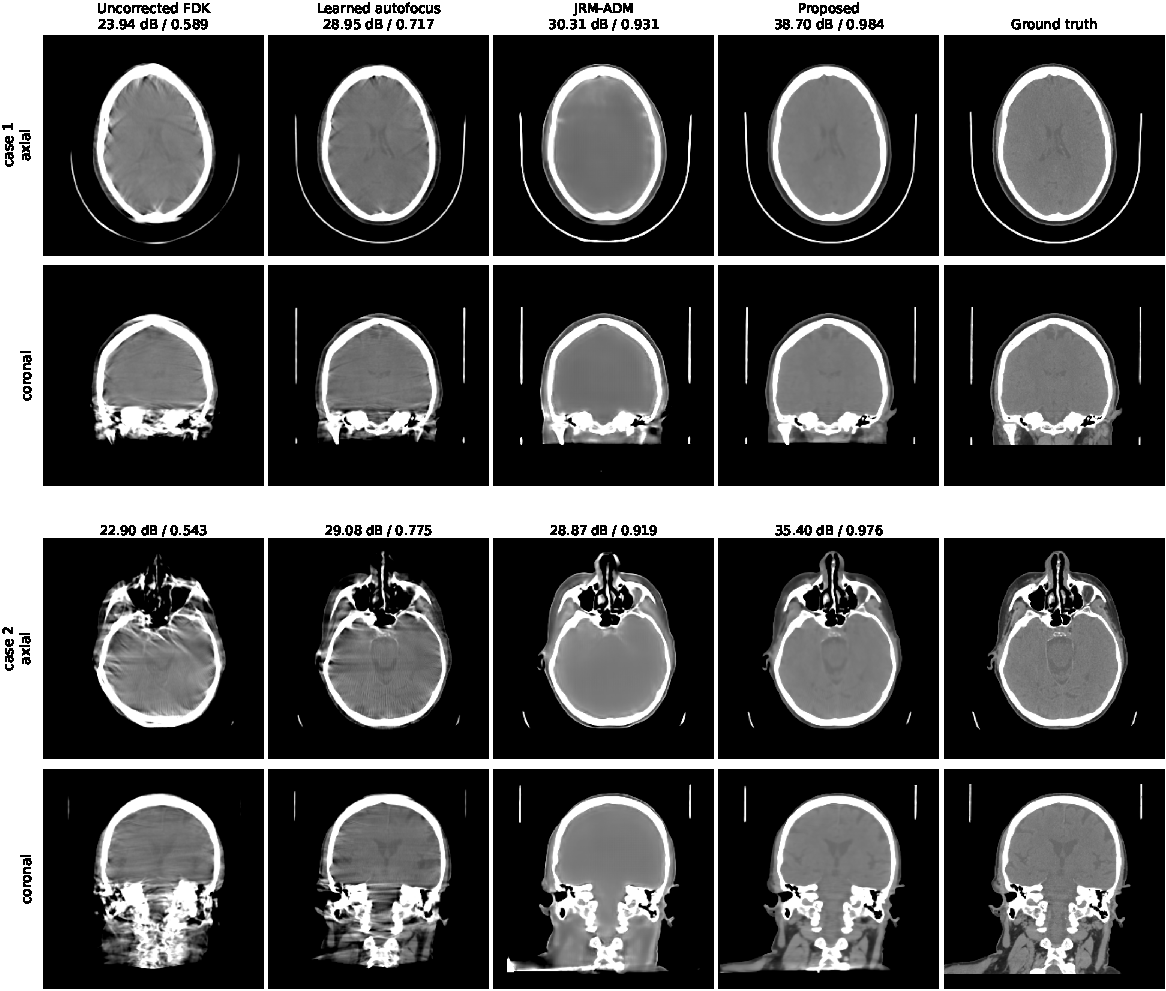
\includegraphics[width=\textwidth]{fig4_bench.pdf}
\caption{Qualitative comparison on two representative test patients (top: mid-brain level;
bottom: skull-base level), brain window; all volumes are rigidly aligned to the ground truth
before slicing, and labels give PSNR\,/\,SSIM against the ground truth. The uncorrected FDK
shows the double contours and streaks of 10\,mm\,/\,10$^\circ$ motion; the autofocus baseline
removes much of the motion but keeps residual streaks; the W3DM prior in our loop
over-smooths and loses texture (the second case is its best in the cohort, and it still
trails the physics bridge in SSIM); the two bridge-trained flow-matching arms recover both
geometry and texture, with the physics bridge sharpest. In the second case the W3DM output's
PSNR is 0.2\,dB above ours despite the blur: the gap sits at the high-contrast bone
interfaces of this skull-base anatomy, which dominate the squared error (38\% of our MSE
falls in the 5\% of voxels above 500\,HU), while soft-tissue error is identical and
smoothing itself is not rewarded (Gaussian-blurring our $x_t$ lowers its PSNR); SSIM, which
normalizes local contrast, ranks the two consistently with the visual impression.}
\label{fig:bench}
\end{figure}

The three loop arms of Table~\ref{tab:main} (rows 3, 4 and 6) form a controlled experiment:
the loop is identical and only the prior differs. Two effects can be read off the $x_t$
column.

\textbf{Effect of the prior class ($+8.5$\,dB).} Replacing the flow-matching prior with the
retrained W3DM diffusion prior costs 8.52\,dB and 0.102 SSIM (30/30 patients,
$p=1.9\times10^{-9}$). The mechanism is visible in the coupling of the loop: the diffusion
prior, trained on clean images only, must be reached through a renoising adapter and pulls
the iterate toward its clean-image manifold, which degrades the intermediate images the
estimator fits on; the motion estimate deteriorates accordingly (Table~\ref{tab:motion}),
which in turn weakens the data step. A bridge-trained prior needs no adapter, because the
states the loop visits are its training distribution. The validation sweep predicted a gap of
about 9\,dB before the test cohort was run, and the cohort reproduced it.

\textbf{Effect of the bridge physics ($+1.4$\,dB).} The pixel-linear bridge arm, trained with
an identical recipe between identical endpoints, lands 1.38\,dB and 0.012 SSIM behind the
physics bridge (27/30 patients, $p=1.6\times10^{-7}$). Notably, the prior-only gap is small
(25.51 versus 25.16\,dB in validation ODE sampling, a difference of $+0.35$\,dB); the loop
amplifies it roughly four-fold, because a slightly better intermediate image buys a better
motion fit (0.28 versus 0.42\,mm in Table~\ref{tab:motion}), which buys a cleaner data step,
compounding over the 50 sweeps. Training on the curve of real FDK reconstructions, with the
exact operator tangent as supervision, is what the additional margin comes from.

Because most of the scored region is air, which inflates PSNR for every method, we
re-scored all four deliverables inside a body region of interest (a mask built from the
ground truth at $-500$\,HU, hole-filled so enclosed sinuses and mastoids count as body, and
reduced to the largest connected component, which also removes the patient table; the
alignment is unchanged). Every conclusion is preserved and the margins hold: our $x_t$
reaches 32.2\,$\pm$\,1.8\,dB\,/\,0.975\,$\pm$\,0.014 against 30.7\,/\,0.965 for the linear
bridge (23--24/30 patients), 24.3\,/\,0.865 for the W3DM prior (29--30/30) and
25.2\,/\,0.880 for the autofocus output (30/30 on both metrics; all $p \le 8\times10^{-5}$).
The isolated PSNR inversion of Fig.~\ref{fig:bench} (second case) persists within the body
ROI on that one patient and remains a 29/30 win cohort-wide.

Fig.~\ref{fig:bench} shows two representative patients across all methods. For completeness, we
also ran our data through the native JRM-ADM pipeline (their solver, grid and retrained
prior, with the operator correspondence cross-checked to 0.16\% on the sinogram). At roughly
4.6 hours per patient it had completed 3 of 30 patients at the time of writing; on those, its
recovered-motion FDK is within 0.5\,dB of ours, consistent with the picture that motion
estimation is near-saturated across methods and the differences concentrate in the prior. The
full native cohort will be reported when complete.

\section{Discussion}
\label{sec:discussion}

The freedom to choose the transport path is what flow matching contributes to this problem.
The intermediate states of the proposed bridge are the images a correction loop actually
passes through, so the prior remains well-defined at every iterate and supplies the update
direction that a joint recovery of image and motion requires. A conventional generative prior
does not have this property, and the unified-loop comparison quantifies what the difference
is worth ($+8.5$\,dB), separately from the contribution of the physics-consistent bridge
shape ($+1.4$\,dB).

The comparisons also clarify where the remaining problem lives. At 10\,mm\,/\,10$^\circ$,
the proposed loop recovers the motion so accurately that the reconstruction at the estimated
poses is nearly indistinguishable from the reconstruction at the true poses (0.980 SSIM
against the oracle), and the autofocus baseline, though behind on this score, still ties our
FDK-class output against the ground truth. The motion-estimation half of the problem appears
close to solved at this amplitude. What separates methods is what they return: an analytic
reconstruction inherits the ceiling of its operator, while the carried iterate surpasses even
the motion-free FDK reference by 3.5\,dB. A practical advantage of returning both is that the
recovered geometry can be verified independently: FDK($\thetahat$) contains no learned
component, so whatever the prior contributes in $x_t$ rests on a trajectory that an analytic
reconstruction confirms.

Several limitations bound these claims. The motion is simulated; to our knowledge no public
real head-CBCT projection data with genuine patient motion exists, so clinical validation is
the essential next step. The motion model is rigid, which suits the skull but not the
mandible or the neck. The autofocus baseline was reimplemented from the paper because most of
its components are unreleased, and although it reproduces the published image-quality
behaviour, its final RPE is somewhat conservative relative to the published value. The native
JRM-ADM transplant is reported on partial evidence. Finally, inference at 9.3 minutes per
patient is dominated by the motion estimator, which is the natural target for acceleration.

\section{Conclusion}
\label{sec:conclusion}

We proposed a blind rigid-motion correction method for head CBCT built on a 3D flow-matching
prior trained along a geometry bridge, with an analytic velocity target and a
predictor-corrector inference loop in which the prior, the motion estimator and the data step
reinforce one another. On 30 held-out CQ500 patients at 10\,mm\,/\,10$^\circ$ peak-to-peak
motion, the method improved every patient, recovered the motion to 0.28\,mm reprojection
error, and produced reconstructions at the estimated poses nearly indistinguishable from
those at the true poses. Paired comparisons on identical data showed that the recovered
motion is more accurate than that of a learned-metric autofocus baseline, and that the
flow-matching prior on the physics-consistent bridge substantially outperforms a
clean-image diffusion prior placed in the same loop. The final iterate exceeded the
motion-free analytic reference, indicating that with the motion essentially solved at this
amplitude, the reconstruction operator itself becomes the limiting factor.

\begin{thebibliography}{19}\small

\bibitem{sisniega17} A.~Sisniega, J.~W. Stayman, J.~Yorkston, J.~H. Siewerdsen, and
W.~Zbijewski, ``Motion compensation in extremity cone-beam CT using a penalized image
sharpness criterion,'' \emph{Phys. Med. Biol.} \textbf{62}(9), 3712--3734 (2017).

\bibitem{thies25} M.~Thies et al., ``A gradient-based approach to fast and accurate head
motion compensation in cone-beam CT,'' \emph{IEEE Trans. Med. Imaging} \textbf{44}(2),
1098--1109 (2025).

\bibitem{huang22} H.~Huang, J.~H. Siewerdsen, W.~Zbijewski, C.~R. Weiss, T.~Ehtiati, and
A.~Sisniega, ``Reference-free learning-based similarity metric for motion compensation in
cone-beam CT,'' \emph{Phys. Med. Biol.} \textbf{67}(12), 125020 (2022).

\bibitem{ko21} Y.~Ko, S.~Moon, J.~Baek, and H.~Shim, ``Rigid and non-rigid motion artifact
reduction in X-ray CT using attention module,'' \emph{Med. Image Anal.} \textbf{67}, 101883
(2021).

\bibitem{pnp13} S.~V. Venkatakrishnan, C.~A. Bouman, and B.~Wohlberg, ``Plug-and-play priors
for model based reconstruction,'' in \emph{IEEE GlobalSIP}, 945--948 (2013).

\bibitem{dds24} H.~Chung, S.~Lee, and J.~C. Ye, ``Decomposed diffusion sampler for
accelerating large-scale inverse problems,'' in \emph{ICLR} (2024).

\bibitem{depaepe25} A.~De Paepe, A.~Bousse, C.~Phung-Ngoc, Y.~Mellak, and D.~Visvikis,
``Adaptive diffusion models for sparse-view motion-corrected head cone-beam CT,''
\emph{IEEE Trans. Radiat. Plasma Med. Sci.} (2025); arXiv:2504.14033.

\bibitem{lipman23} Y.~Lipman, R.~T.~Q. Chen, H.~Ben-Hamu, M.~Nickel, and M.~Le, ``Flow
matching for generative modeling,'' in \emph{ICLR} (2023).

\bibitem{indi23} M.~Delbracio and P.~Milanfar, ``Inversion by direct iteration: an
alternative to denoising diffusion for image restoration,'' \emph{Trans. Mach. Learn. Res.}
(2023).

\bibitem{albergo23} M.~S. Albergo, M.~Goldstein, N.~M. Boffi, R.~Ranganath, and
E.~Vanden-Eijnden, ``Stochastic interpolants with data-dependent couplings,'' arXiv:2310.03725
(2023).

\bibitem{i2sb23} G.-H. Liu, A.~Vahdat, D.-A. Huang, E.~A. Theodorou, W.~Nie, and
A.~Anandkumar, ``I$^2$SB: image-to-image Schr\"odinger bridge,'' in \emph{ICML} (2023).

\bibitem{yang25} T.~Yang, J.~Hu, J.~A. Fessler, and L.~Shen, ``Local patches meet global
context: scalable 3D diffusion priors for computed tomography reconstruction,''
arXiv:2512.18161 (2025).

\bibitem{mueller22} T.~M\"uller, A.~Evans, C.~Schied, and A.~Keller, ``Instant neural
graphics primitives with a multiresolution hash encoding,'' \emph{ACM Trans. Graph.}
\textbf{41}(4), 102 (2022).

\bibitem{leap23} H.~Kim and K.~Champley, ``Differentiable forward projector for X-ray
computed tomography,'' arXiv:2307.05801 (2023); LEAP,
\url{https://github.com/LLNL/LEAP}.

\bibitem{cq500} S.~Chilamkurthy et al., ``Deep learning algorithms for detection of critical
findings in head CT scans: a retrospective study,'' \emph{The Lancet} \textbf{392}(10162),
2388--2396 (2018).

\bibitem{akima70} H.~Akima, ``A new method of interpolation and smooth curve fitting based on
local procedures,'' \emph{J. ACM} \textbf{17}(4), 589--602 (1970).

\bibitem{wdm24} P.~Friedrich, J.~Wolleb, F.~Bieder, A.~Durrer, and P.~C. Cattin, ``WDM: 3D
wavelet diffusion models for high-resolution medical image synthesis,'' in \emph{MICCAI
Workshop on Deep Generative Models}, 11--21 (2024).

\bibitem{sdedit22} C.~Meng, Y.~He, Y.~Song, J.~Song, J.~Wu, J.-Y. Zhu, and S.~Ermon,
``SDEdit: guided image synthesis and editing with stochastic differential equations,'' in
\emph{ICLR} (2022).

\end{thebibliography}

\end{document}
